\documentclass[../main.tex]{subfiles}

\begin{document}

\chapter{Implementation and Enhancements}
\label{chap:Implementation}

\section{Implementation Challenges}
\label{sec:implementation_challenges}

% The available reference decoder used during lab experiments was designed for hard values, where received bits are quantized strictly into 0 or 1.

% In contrast, my decoder was required to operate on soft values (e.g., log-likelihood ratios or confidence levels), which carry reliability information.

% This difference meant that I could not directly reuse the provided implementation but only use it as a conceptual guide.

% Hard-decision algorithms often rely on simple binary operations (XOR, parity checks).

% Soft-decision decoding requires handling probability information, which introduces additional numerical complexity and careful treatment of floating-point operations.

% Ensuring numerical stability (e.g., avoiding underflow/overflow in probability updates) was a challenge.

% Soft-decision decoding (especially min-sum or sum-product algorithms) is computationally heavier compared to hard-decision decoding.

% Choosing efficient data structures and approximations was necessary to keep the implementation practical.

During the development of the \gls{ldpc} decoder, several challenges emerged, mainly due to differences between the available reference implementation and the requirements of the final system. 
The reference decoder, which had been provided in the context of laboratory exercises, was designed for hard-decision decoding, while the target application demanded a soft-decision decoder. 
This discrepancy significantly shaped the implementation process.

The first challenge stemmed from the fundamental difference between hard and soft inputs. 
In the laboratory implementation, the decoder operated on hard values, i.e., binary decisions of 0 or 1 obtained after thresholding the received signal. 
This approach simplifies the decoding process but disregards reliability information contained in the received data. 
In contrast, the target system required the handling of soft values, typically expressed in the form of \glspl{llr}. 
These values do not only indicate whether a bit is likely to be a zero or one, but also quantify the confidence in this decision.
As a result, the decoder needed to process real-valued inputs and propagate reliability information throughout the iterative decoding steps.

\begin{equation}
L(y) = \ln\!\left(\frac{P(x=0\mid y)}{P(x=1\mid y)}\right).
\label{eq:llr_def}
\end{equation}

\vspace{1em}
\begin{figure}[htbp]
  \centering
  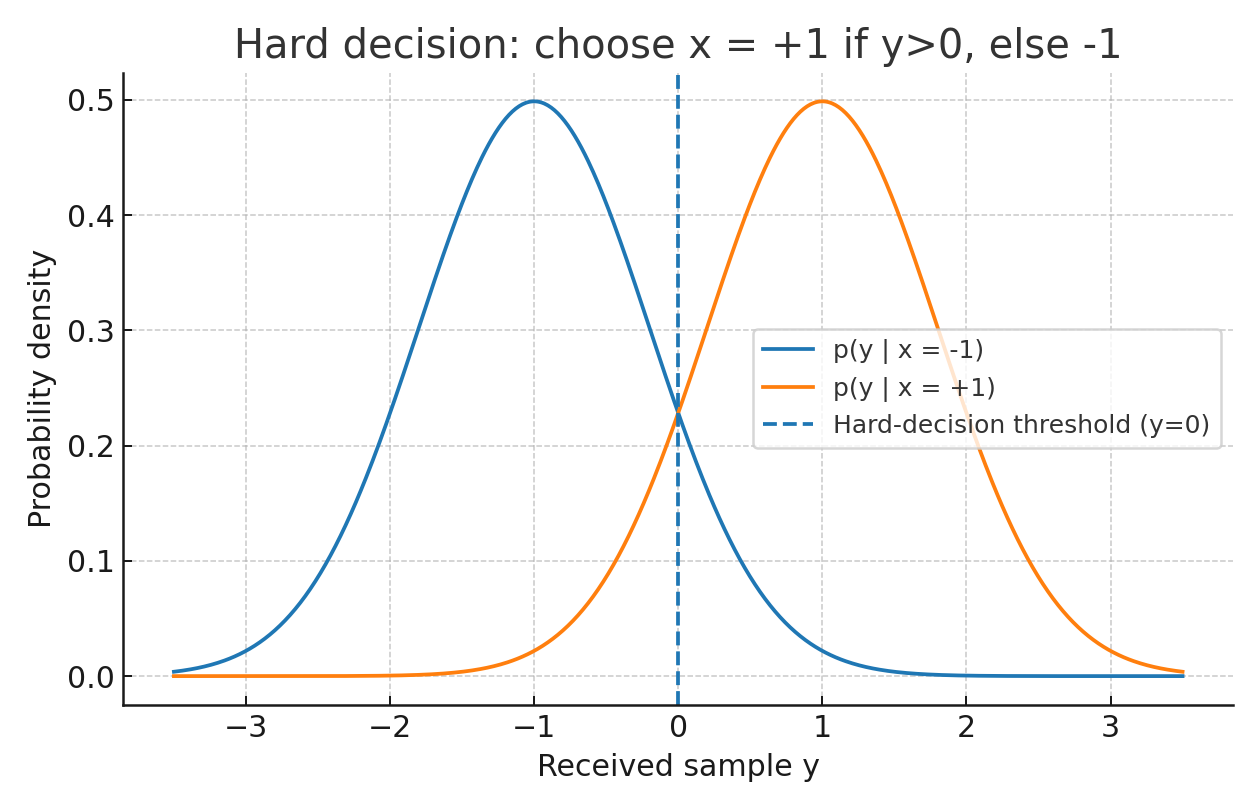
\includegraphics[width=0.85\linewidth]{figs/ldpc_hard_vs_soft_pdfs.png}
  \caption{BPSK over AWGN: conditional likelihoods \(p(y\mid x=\pm1)\) and the hard-decision threshold at \(y=0\).
  Hard decisions select \(x=+1\) when \(y>0\) and \(x=-1\) otherwise, discarding reliability.
  Soft decisions retain confidence via the magnitude of the LLR in \eqref{eq:llr_def}.}
  \label{fig:hard_soft_threshold}
\end{figure}
\vspace{1em}

This naturally led to the second major challenge: adapting the decoding algorithm to support soft values. 
Hard-decision decoding relies on simple binary operations, such as XOR computations for parity checks, which are relatively straightforward to implement. 
In the case of soft-decision decoding, however, the update rules involve probability-domain or log-domain computations.
For example, the check-node and variable-node updates in the sum-product or min-sum algorithms rely on nonlinear functions of the input \glspl{llr}. 
Implementing these operations required careful consideration of numerical stability, as certain expressions are prone to underflow, overflow, or loss of precision in floating-point arithmetic. 
Approximation strategies, such as the min-sum approach, had to be evaluated as a means of reducing complexity while maintaining decoding performance.

A third challenge arose from the increased computational and resource requirements of soft-decision decoding. 
Whereas the hard-decision algorithm could be implemented with simple bit-wise operations, the soft-decision variant introduces additional computational burden due to the need for iterative updates of real-valued messages. 
This has implications for both execution time and memory usage. 
Designing data structures that allowed efficient storage and retrieval of messages between check and variable nodes was therefore an important step. 
Moreover, it was necessary to balance algorithmic accuracy with practical constraints, ensuring that the implementation remained feasible for the intended use case.

In summary, the transition from a hard-decision reference implementation to a fully functional soft-decision decoder introduced challenges at both the algorithmic and implementation level. 
The handling of real-valued inputs, the numerical stability of update rules, and the increased computational demands all required tailored solutions. 
These adaptations ultimately ensured that the developed decoder could achieve the desired performance under realistic channel conditions.

\section{Decoder design and Architecture}
\label{sec:decoder_design}

% In your preamble (if not already present):
% \usepackage{amsmath,amssymb}
% \usepackage{tikz}
% \usetikzlibrary{arrows.meta,positioning,fit,calc,shapes,decorations.pathreplacing}
% \usepackage{booktabs}
% \usepackage{siunitx}

\subsection{Design and Architecture}
\label{subsec:design_architecture}

Scope of implementation:

Only the core LDPC decoder was implemented.

Other parts of the decoding chain such as reverse scrambling, inverse rate matching, and CRC check were left out but are necessary in a full system.

Input / Output interfaces:

Input: Log-likelihood ratios (LLRs) for each codeword bit (soft values).

Output: Configurable as either

hard decisions $\hat{x}_v \in \{0,1\}$ or soft output LLRs ($L_{APP}$) for use by later modules (e.g., CRC check).

Control parameters: maximum iterations, decoding schedule (layered vs. flooding), stopping criteria.

Core architecture:

Based on iterative message passing on the Tanner graph.

    Separation of concerns

    Variable Node (VN) processing: combines channel LLRs with incoming check node messages.

    Check Node (CN) processing: computes outgoing messages using Sum-Product or Min-Sum rules.

        Iteration controller: orchestrates scheduling, stopping conditions, and updates.

    Edge message buffers store $L_{v \to c}$ and $L_{c \to v}$ efficiently.

Implemented algorithms:

Implemented four variants of message-passing decoding:

Sum-Product Algorithm (SPA)

Min-Sum (MS)

Offset Min-Sum (OMS)

Normalized Min-Sum (NMS)

Each trades off complexity and performance differently.

Comparative performance evaluation of these algorithms will be presented in the next chapter.

Scheduling:

Layered decoding was chosen (row-by-row updates) to accelerate convergence.

Alternative flooding schedule possible but less efficient.

Numerical considerations:

Floating-point arithmetic for prototyping, with optional fixed-point representation (Q-format) if hardware mapping is needed.

Min-Sum approximation used to reduce complexity and improve numerical stability.

Clipping of extreme LLRs to prevent overflow.

Integration with external chain:

Decoder designed to be modular, with clean interfaces for upstream (inverse rate matching) and downstream (CRC check).

Extensible configuration for base graph selection, lifting factor Z, and algorithm choice.

With the design and implementation of the core LDPC decoder established, including support for multiple decoding algorithms (SPA, MS, OMS, NMS) and a modular architecture that integrates seamlessly into the larger decoding chain, the next step is to evaluate its performance. 
The following chapter, Experimental Results and Analysis, presents a comparative study of the implemented algorithms under different channel conditions, highlighting their trade-offs in terms of error-correction capability, computational complexity, and convergence behavior.

\end{document}